\section{Pregunta N$^{\circ}$4\qquad Andre Gilmer Santos Felix}

\begin{frame}
    \begin{theorem}[Binomio de Newton]
        Si $a,b\in\mathbb{C}$, entonces
        \begin{math}
            \forall n\in\mathbb{N}\cup\left\{0\right\}:
        \end{math}

        \begin{equation}\label{eq:binomial}
            \left(a+b\right)^{n}=
            \sum\limits_{j=0}^{n}
            \dbinom{n}{j}
            a^{j}
            b^{n-j}.
        \end{equation}
    \end{theorem}

    Derivando~\eqref{eq:binomial} con respecto de $a$, tenemos
    \begin{align}
        \diffp{
            \alert{
                \left(a+b\right)^{n}
            }
        }{a}                    & =
        \diffp{
            \alert{
                \sum\limits_{j=0}^{n}
                \dbinom{n}{j}
                a^{j}
                b^{n-j}
            }
        }{a}.  \notag               \\
        n\left(a+b\right)^{n-1} & =
        \sum\limits_{j=0}^{n}
        \dbinom{n}{j}
        b^{n-j}
        \diffp{
            \alert{
                a^{j}
            }
        }{a}.   \notag              \\
        \alert{a}
        n\left(a+b\right)^{n-1}
                                & =
        \alert{a}
        \sum\limits_{j=0}^{n}
        \dbinom{n}{j}
        \alert{ja^{j-1}}
        b^{n-j}.      \notag        \\
        \label{eq:binomial_I}
        \Aboxed{
            a\left(a+b\right)^{n-1}
                                & =
            \sum\limits_{j=0}^{n}
            \dfrac{j}{n}
            \dbinom{n}{j}
            a^{j}
            b^{n-j}.
        }
    \end{align}
\end{frame}

\begin{frame}
    Derivando~\eqref{eq:binomial} dos veces con respecto de $a$,
    tenemos
    \begin{align}
        \diffp[2]{
            \alert{
                \left(a+b\right)^{n}
            }
        }{a}                   & =
        \diffp[2]{
            \alert{
                \sum\limits_{j=0}^{n}
                \dbinom{n}{j}
                a^{j}
                b^{n-j}
            }
        }{a}.   \notag             \\
        \diffp{
            \alert{
                n\left(a+b\right)^{n-1}
            }
        }{a}                   & =
        \diffp{
            \alert{
                \sum\limits_{j=0}^{n}
                \dbinom{n}{j}
                ja^{j-1}
                b^{n-j}
            }
        }{a}.         \notag       \\
        n\left(n-1\right)
        \left(a+b\right)^{n-2} & =
        \sum\limits_{j=0}^{n}
        \dbinom{n}{j}
        b^{n-j}
        j
        \diffp{
            \alert{
                a^{j-1}
            }
        }{a}.               \notag \\
        \alert{
            \dfrac{a^{2}}{n^{2}}
        }
        n\left(n-1\right)
        \left(a+b\right)^{n-2} & =
        \alert{
            \dfrac{a^{2}}{n^{2}}
        }
        \sum\limits_{j=0}^{n}
        \dbinom{n}{j}
        b^{n-j}
        j
        \alert{
            \left(j-1\right)
            a^{j-2}
        }.                \notag   \\
        \dfrac{n-1}{n}
        a^{2}
        \left(a+b\right)^{n-2}
                               & =
        \sum\limits_{j=0}^{n}
        \dfrac{j\left(j-1\right)}{n^{2}}
        \dbinom{n}{j}
        a^{j}
        b^{n-j}.          \notag   \\
        \label{eq:binomial_II}
        \Aboxed{
            \left(1-\dfrac{1}{n}\right)
            a^{2}
            \left(a+b\right)^{n-2}
                               & =
            \sum\limits_{j=0}^{n}
            \left(
            \dfrac{j^{2}}{n^{2}}-
            \dfrac{j}{n^{2}}
            \right)
            \dbinom{n}{j}
            a^{j}
            b^{n-j}.
        }
    \end{align}
\end{frame}

\begin{frame}
    Definimos
    \begin{math}
        B_{n,j}\left(x\right)\coloneqq
        \dbinom{n}{j}
        x^{j}
            {\left(1-x\right)}^{n-j}
    \end{math}
    para cualquier
    \begin{math}
        \forall j\in\left\{0,\dotsc,n\right\}
    \end{math}.
    Si sustituimos $a=\alert{x}$ y $b=\alert{1-x}$
    en~\eqref{eq:binomial},~\eqref{eq:binomial_I}
    y~\eqref{eq:binomial_II}
    \begin{align}
        \left(\alert{x}+\alert{1-x}\right)^{n} & =
        \sum\limits_{j=0}^{n}
        \dbinom{n}{j}
        \alert{x}^{j}
        {\left(\alert{1-x}\right)}^{n-j}. \notag   \\
        \Aboxed{
        1                                      & =
            \sum\limits_{j=0}^{n}
            B_{n,j}\left(x\right).
        }                                          \\
        \alert{x}\left(\alert{x}+\alert{1-x}\right)^{n-1}
                                               & =
        \sum\limits_{j=0}^{n}
        \dfrac{j}{n}
        \dbinom{n}{j}
        \alert{x}^{j}
        {\left(\alert{1-x}\right)}^{n-j}. \notag   \\
        \Aboxed{
            x
                                               & =
            \sum\limits_{j=0}^{n}
            \dfrac{j}{n}
            B_{n,j}\left(x\right).
        }                                          \\
        \left(1-\dfrac{1}{n}\right)
        \alert{x}^{2}
        \left(\alert{x}+\alert{1-x}\right)^{n-2}
                                               & =
        \sum\limits_{j=0}^{n}
        \left(
        \dfrac{j^{2}}{n^{2}}-
        \dfrac{j}{n^{2}}
        \right)
        \dbinom{n}{j}
        \alert{x}^{j}
        {\left(\alert{1-x}\right)}^{n-j}.
        \notag                                     \\
        \left(1-\dfrac{1}{n}\right)
        x^{2}
                                               & =
        \sum\limits_{j=0}^{n}
        \left(
        \dfrac{j^{2}}{n^{2}}-
        \dfrac{j}{n^{2}}
        \right)
        B_{n,j}\left(x\right)=
        \sum\limits_{j=0}^{n}
        \dfrac{j^{2}}{n^{2}}
        B_{n,j}\left(x\right)-
        \frac{1}{n}
        \alert{
            \sum\limits_{j=0}^{n}
            \dfrac{j}{n}
            B_{n,j}\left(x\right)
        }.
        \notag                                     \\
        \Aboxed{
            \left(1-\dfrac{1}{n}\right)
            x^{2}+
            \dfrac{\alert{x}}{n}
                                               & =
            \sum\limits_{j=0}^{n}
            \dfrac{j^{2}}{n^{2}}
            B_{n,j}\left(x\right).
        }
    \end{align}
\end{frame}

\begin{frame}
	\begin{enumerate}\setcounter{enumi}{3}
		\item

		      Demuestre que
		      \begin{math}
			      \forall n\in\mathbb{N}:
			      B_{n}\left(x\right)=
			      \left(\dfrac{n-1}{n}\right)x^{2}+
			      \dfrac{1}{n}x
		      \end{math}
		      y determine un $n_{0}$ tal que
		      \begin{math}
			      \left|
			      B_{n_{0}}\left(x\right)-
			      x^{2}
			      \right|\leq
			      10^{-6}
		      \end{math}
		      se satisface para todo $x\in\left[0,1\right]$.
	\end{enumerate}

	\begin{solution}
		Sean $x\in\left[0,1\right]$ y $n\in\mathbb{N}$, definimos
		\begin{math}
			B_{n}\left(x\right)\coloneqq
			\sum\limits_{j=0}^{n}
			\dfrac{j^{2}}{n^{2}}
			B_{n,j}\left(x\right)
		\end{math}
		para cualquier
		\begin{math}
			\forall n\in\mathbb{N}
		\end{math}.

		\begin{figure}[ht!]
			\centering
			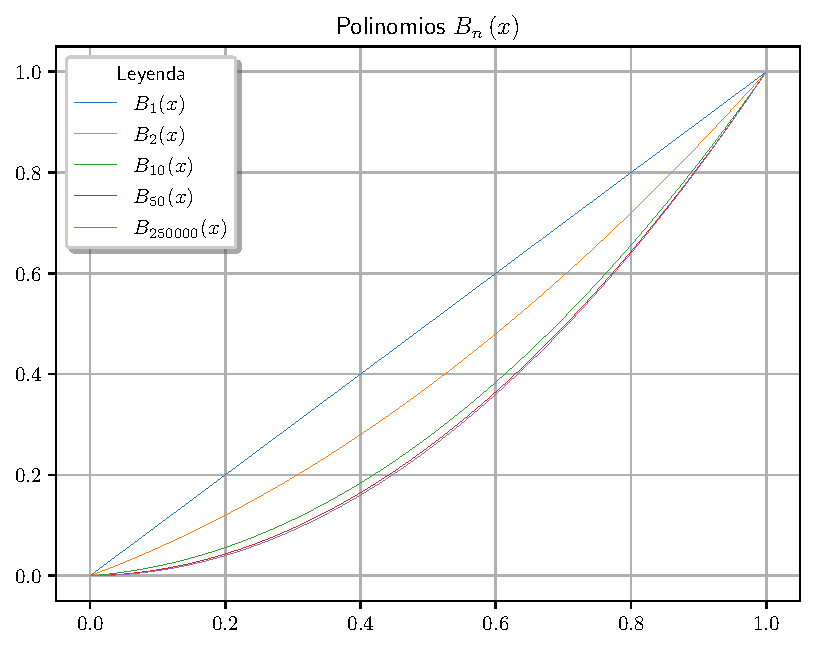
\includegraphics[width=.55\paperwidth]{p4}
		\end{figure}
	\end{solution}
\end{frame}

\begin{frame}
	\begin{solution}
		Sea $n\in\mathbb{N}$ y $x\in\left[0,1\right]$.

		\begin{alignat*}{2}
			0             & \leq x                                                           &  & \leq 1.            \\
			-\dfrac{1}{2} & \leq x-\dfrac{1}{2}                                              &  & \leq \dfrac{1}{2}. \\
			0             & \leq {\left(x-\dfrac{1}{2}\right)}^{2}                           &  & \leq \dfrac{1}{4}. \\
			-\dfrac{1}{4} & \leq {\left(x-\dfrac{1}{2}\right)}^{2}-\dfrac{1}{4}              &  & \leq 0.            \\
			0             & \leq \left|{\left(x-\dfrac{1}{2}\right)}^{2}-\dfrac{1}{4}\right| &  & \leq \dfrac{1}{4}.
		\end{alignat*}

		Por lo tanto,
		\begin{math}
			\exists n_{0}\in\mathbb{N}
		\end{math}
		tal que
		\begin{math}
			\forall x\in\left[0,1\right]:
			\left|B_{n_{0}}\left(x\right)-x^{2}\right|\leq
			10^{-6}
		\end{math}.

		\begin{align*}
			\left|
			\alert{
				B_{n_{0}}\left(x\right)
			}
			-x^{2}
			\right| & =
			\left|
			\alert{
			\left(\dfrac{n-1}{n}\right)x^{2}+
			\dfrac{1}{n}x
			}
			-x^{2}
			\right|=
			\left|
			x^{2}\left(1-\dfrac{1}{n}-1\right)+\dfrac{x}{n}
			\right|=
			\left|
			-\dfrac{x^{2}}{n}+\dfrac{x}{n}
			\right|
			=\left|
			\dfrac{1}{n}
			\left(x-x^{2}\right)
			\right|     \\
			        & =
			\dfrac{1}{n}
			\left|
			x^{2}-x
			\right|=
			\dfrac{1}{n}
			\left|
			{\left(x-\dfrac{1}{2}\right)}^{2}-
			\dfrac{1}{4}
			\right|\leq
			10^{-6}.
		\end{align*}

		Entonces,
		\begin{math}
			\dfrac{1}{4n_{0}}=10^{-6}\iff n_{0}=250000
		\end{math}.
	\end{solution}
\end{frame}